\section{Projected Results}

\subsection{Kinematic Coverage}

\begin{figure}[!ht]
 \begin{center}
      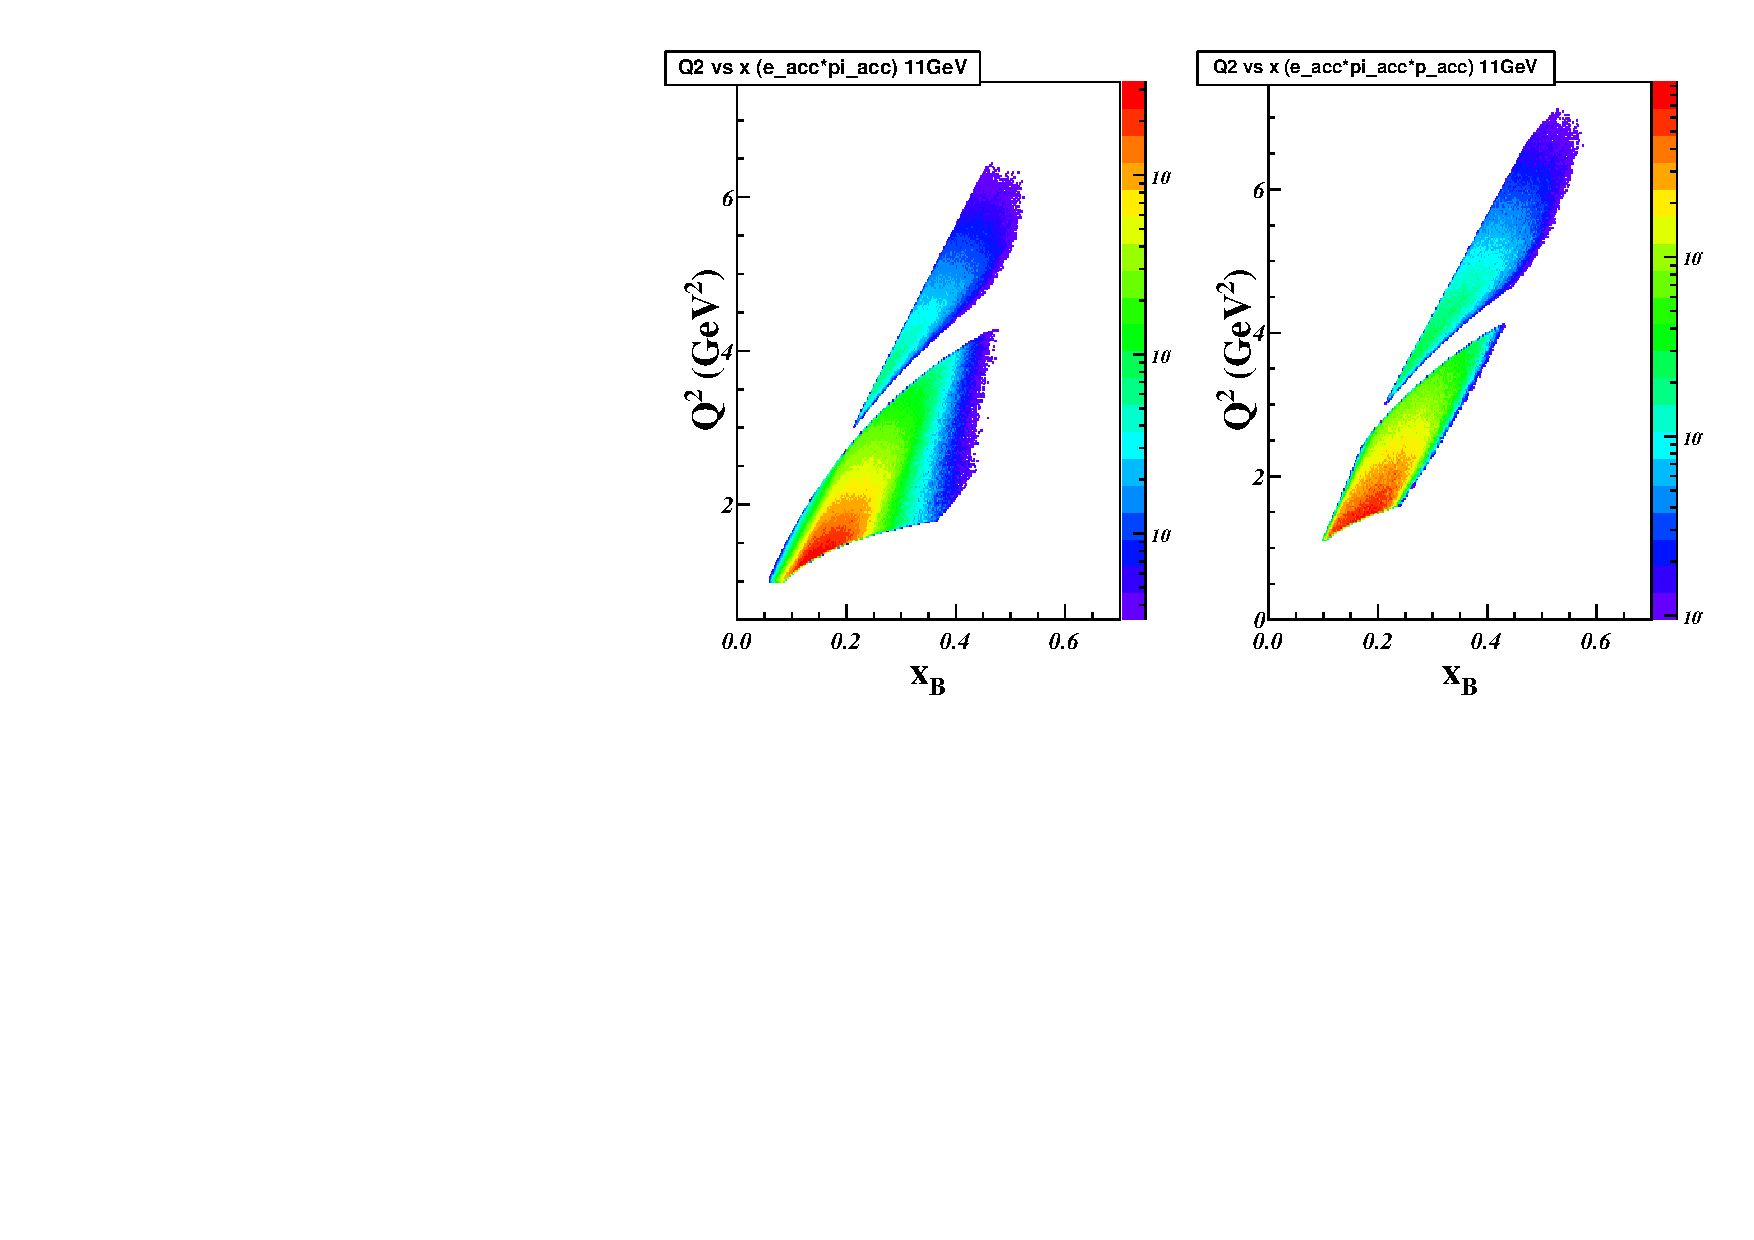
\includegraphics[type=pdf,
        ext=.pdf,read=.pdf,width=0.6\textwidth]{./figures/E11_Q2_x_epip_Q2gt1}
 \caption[The kinematic coverage at different acceptances.]{\footnotesize{The
     kinematic coverage at different acceptances at 11~GeV. The left plot
     shows the coverage when detecting all recoil protons, while the right plot
     shows the coverage with proton detection by existing SoLID
     detectors. Colors correspond to rates (Hz) in log scale.}}
  \label{kin_cor}
  \end{center}
\end{figure}

%\begin{figure}[!ht]
% \begin{center}
%    \subfloat[w/ $\mathrm{Q^{2}>1~GeV^{2}}$ cut]{
%      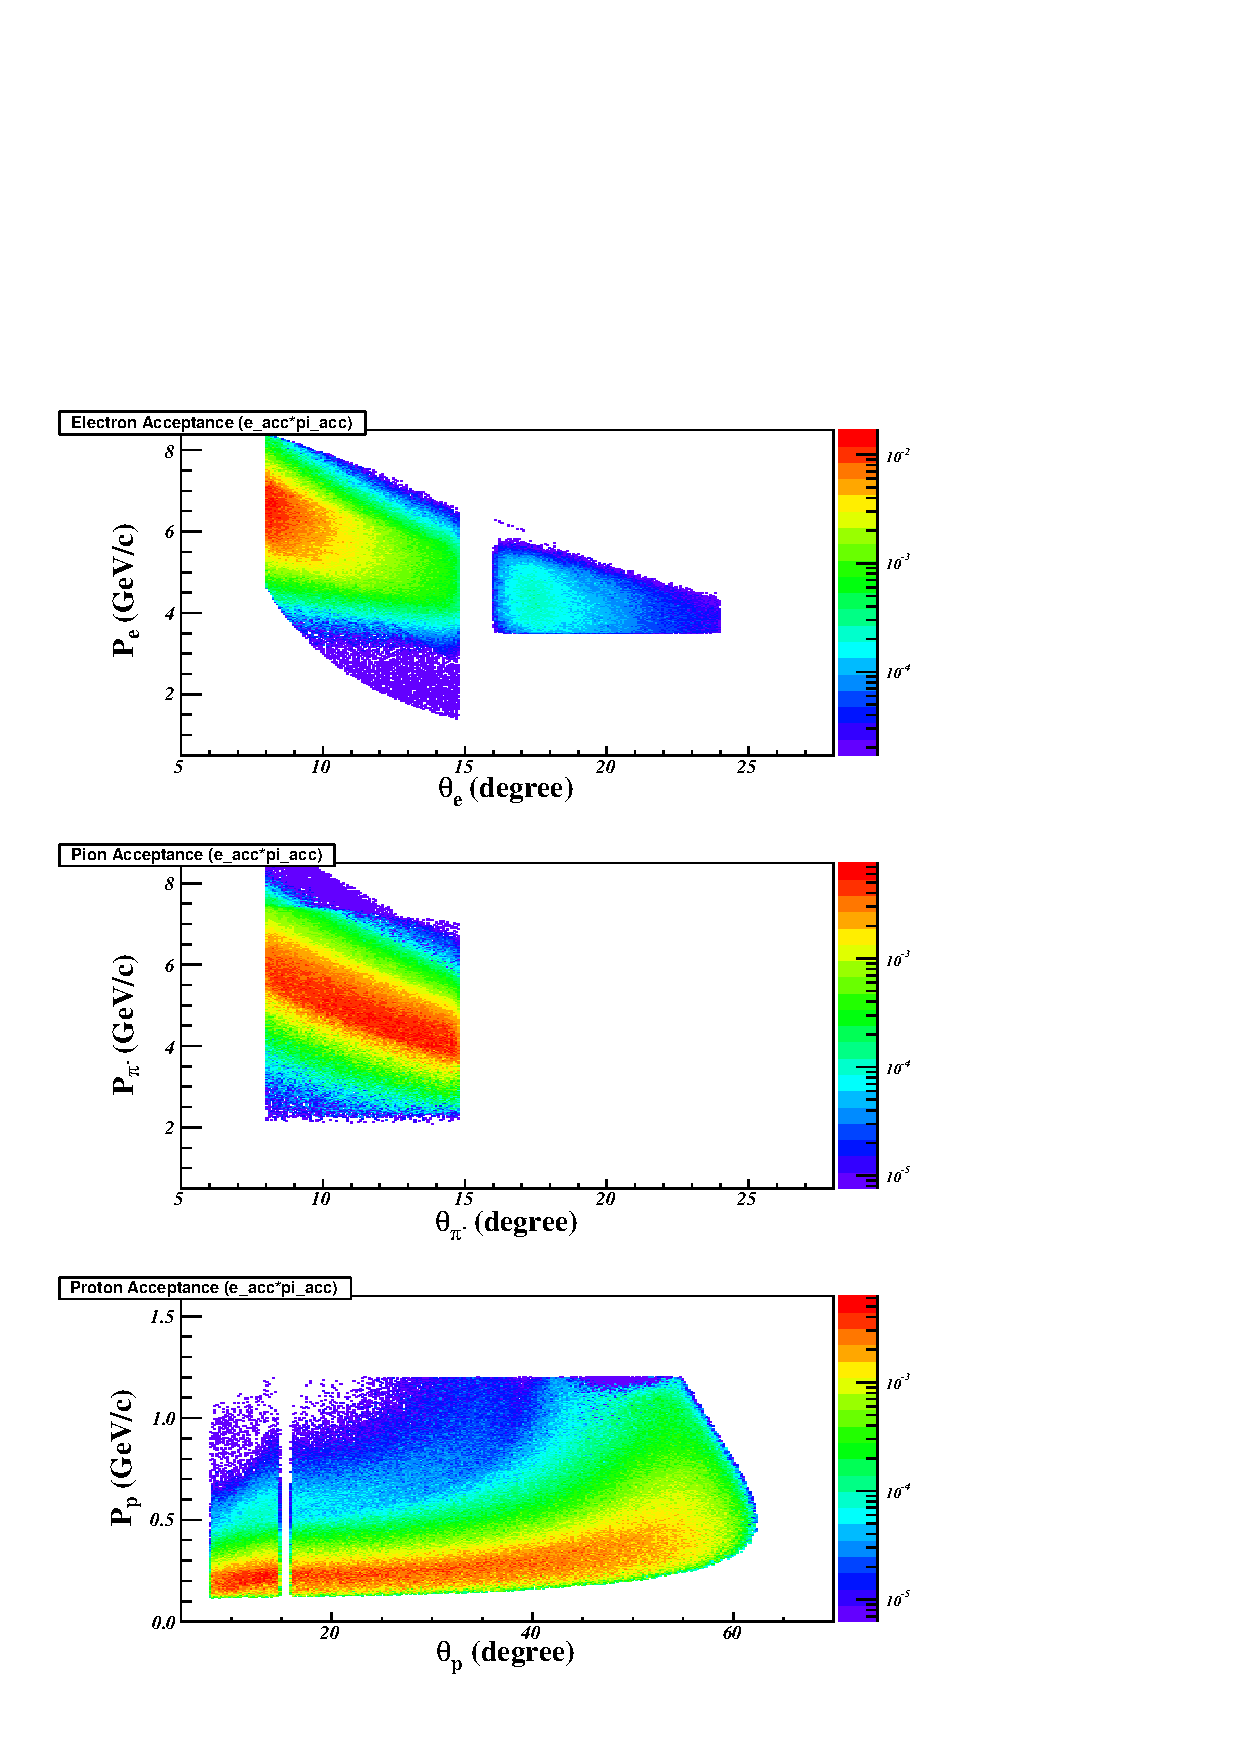
\includegraphics[type=pdf, ext=.pdf,read=.pdf,width=0.35\textwidth]{./figures/E11_acc_epi}
%    }
%     \subfloat[w/ $\mathrm{Q^{2}>4~GeV^{2}}$ cut]{
%      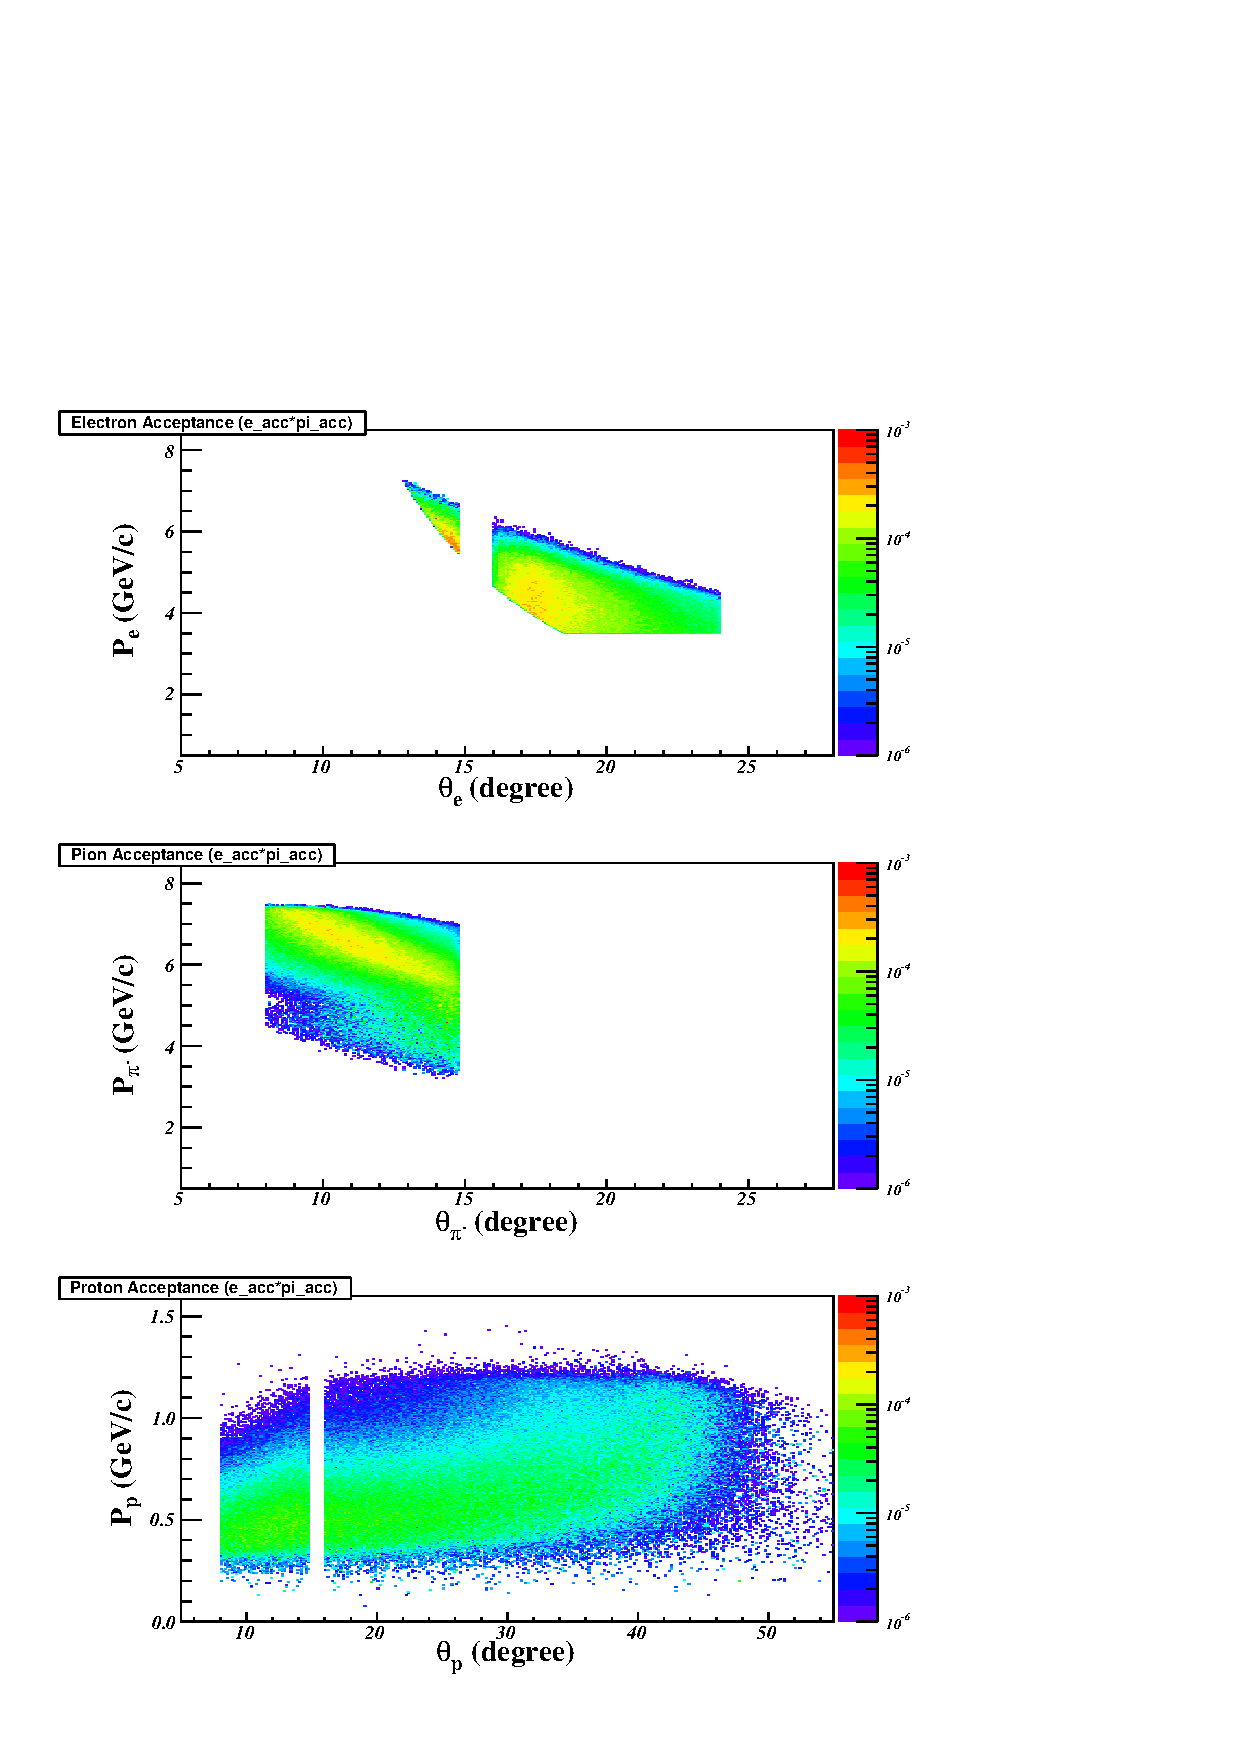
\includegraphics[type=pdf, ext=.pdf,read=.pdf,width=0.35\textwidth]{./figures/E11_acc_epi_Q2gt4}
%    }
%   \caption[The acceptance of the momenta and scattering angles for electrons, $\pi^{-}$ and protons]{\footnotesize{The acceptance of the momenta and polar angles at two different $\mathrm{Q^{2}}$ cuts. In each panel, the top, middle and bottom plots are for electrons, $\pi^{-}$ and protons, respectively. The distribution of protons is given by assuming we detect all recoil protons. Colors correspond to rates (Hz) in log scale.}}
%  \label{p_theta}
%  \end{center}
%\end{figure}
%\begin{figure}[!ht]
% \begin{center}
%    \subfloat[w/ $\mathrm{Q^{2}>1~GeV^{2}}$ cut]{
%      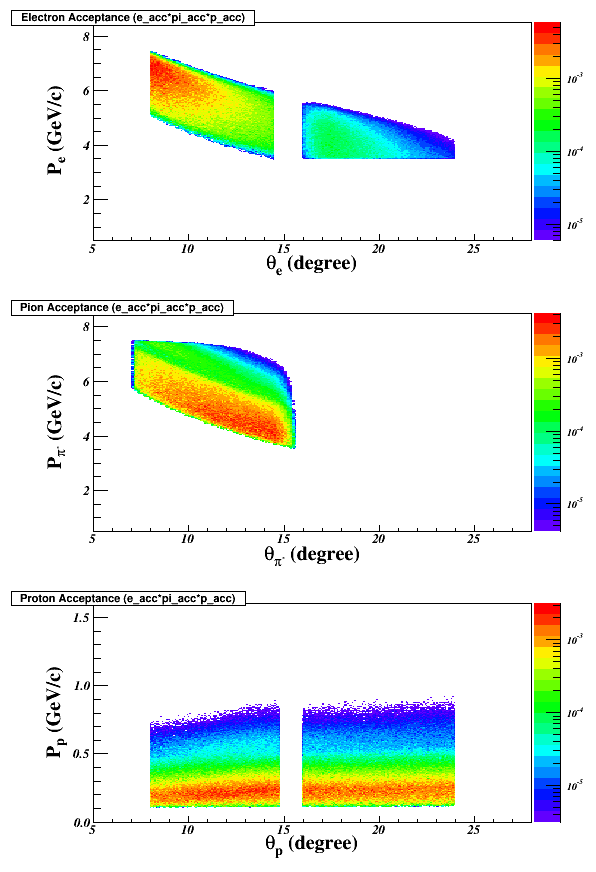
\includegraphics[type=pdf, ext=.pdf,read=.pdf,width=0.35\textwidth]{./figures/E11_acc_epip}
%    }
%     \subfloat[w/ $\mathrm{Q^{2}>4~GeV^{2}}$ cut]{
%      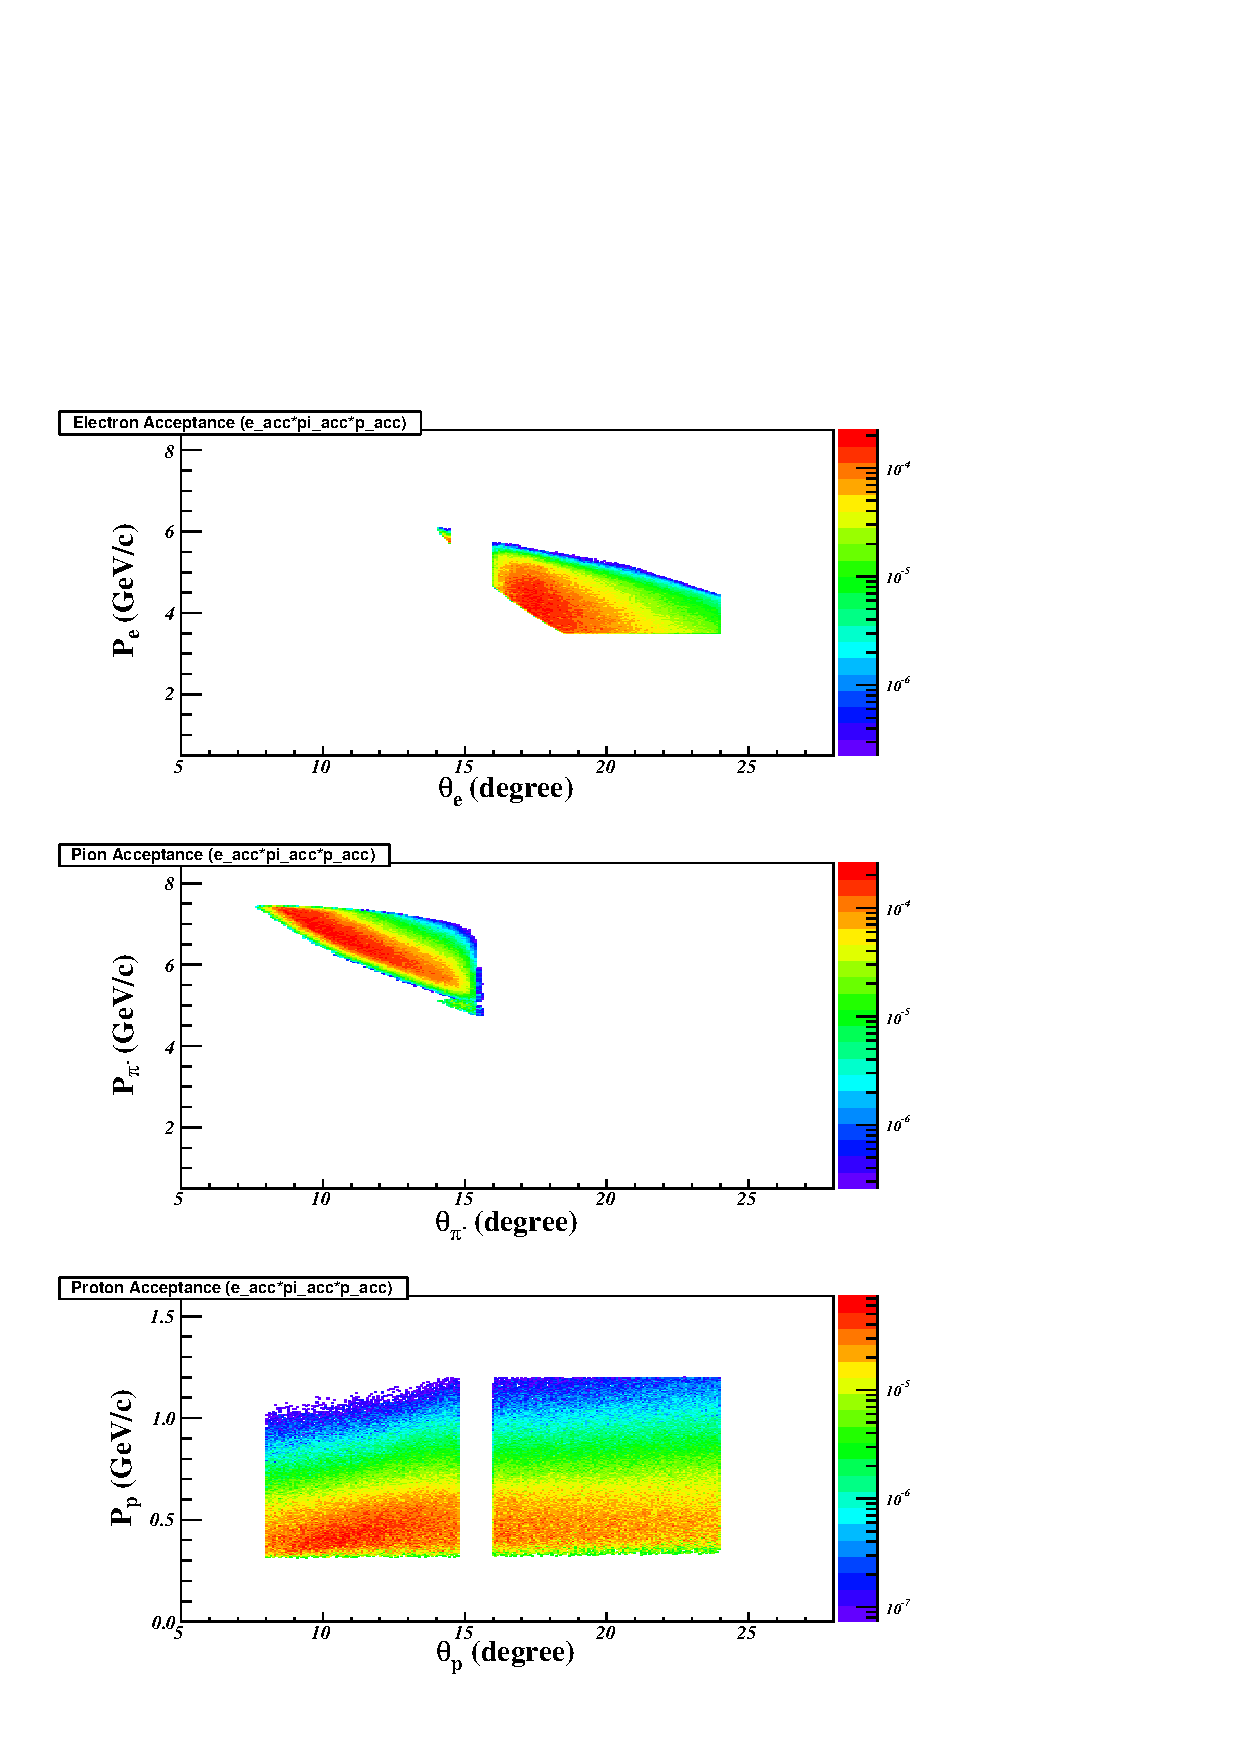
\includegraphics[type=pdf, ext=.pdf,read=.pdf,width=0.35\textwidth]{./figures/E11_acc_epip_Q2gt4}
%    }
%   \caption[The acceptance of the momenta and scattering angles for electrons, $\pi^{-}$ and protons when only detecting small angle protons]{\footnotesize{The acceptance of the momenta and polar angles  at two different $\mathrm{Q^{2}}$ cuts  when only detecting small angle protons with the existing SoLID detectors. In each panel, the top, middle and bottom plots are for electrons, $\pi^{-}$ and protons, respectively. The distribution of protons is given by assuming we detect all recoil protons. Colors correspond to rates (Hz) in log scale.}}
%  \label{p_theta1}
%  \end{center}
%\end{figure}

\begin{figure}[!ht]
 \begin{center}
    \subfloat[w/ PRD]{
      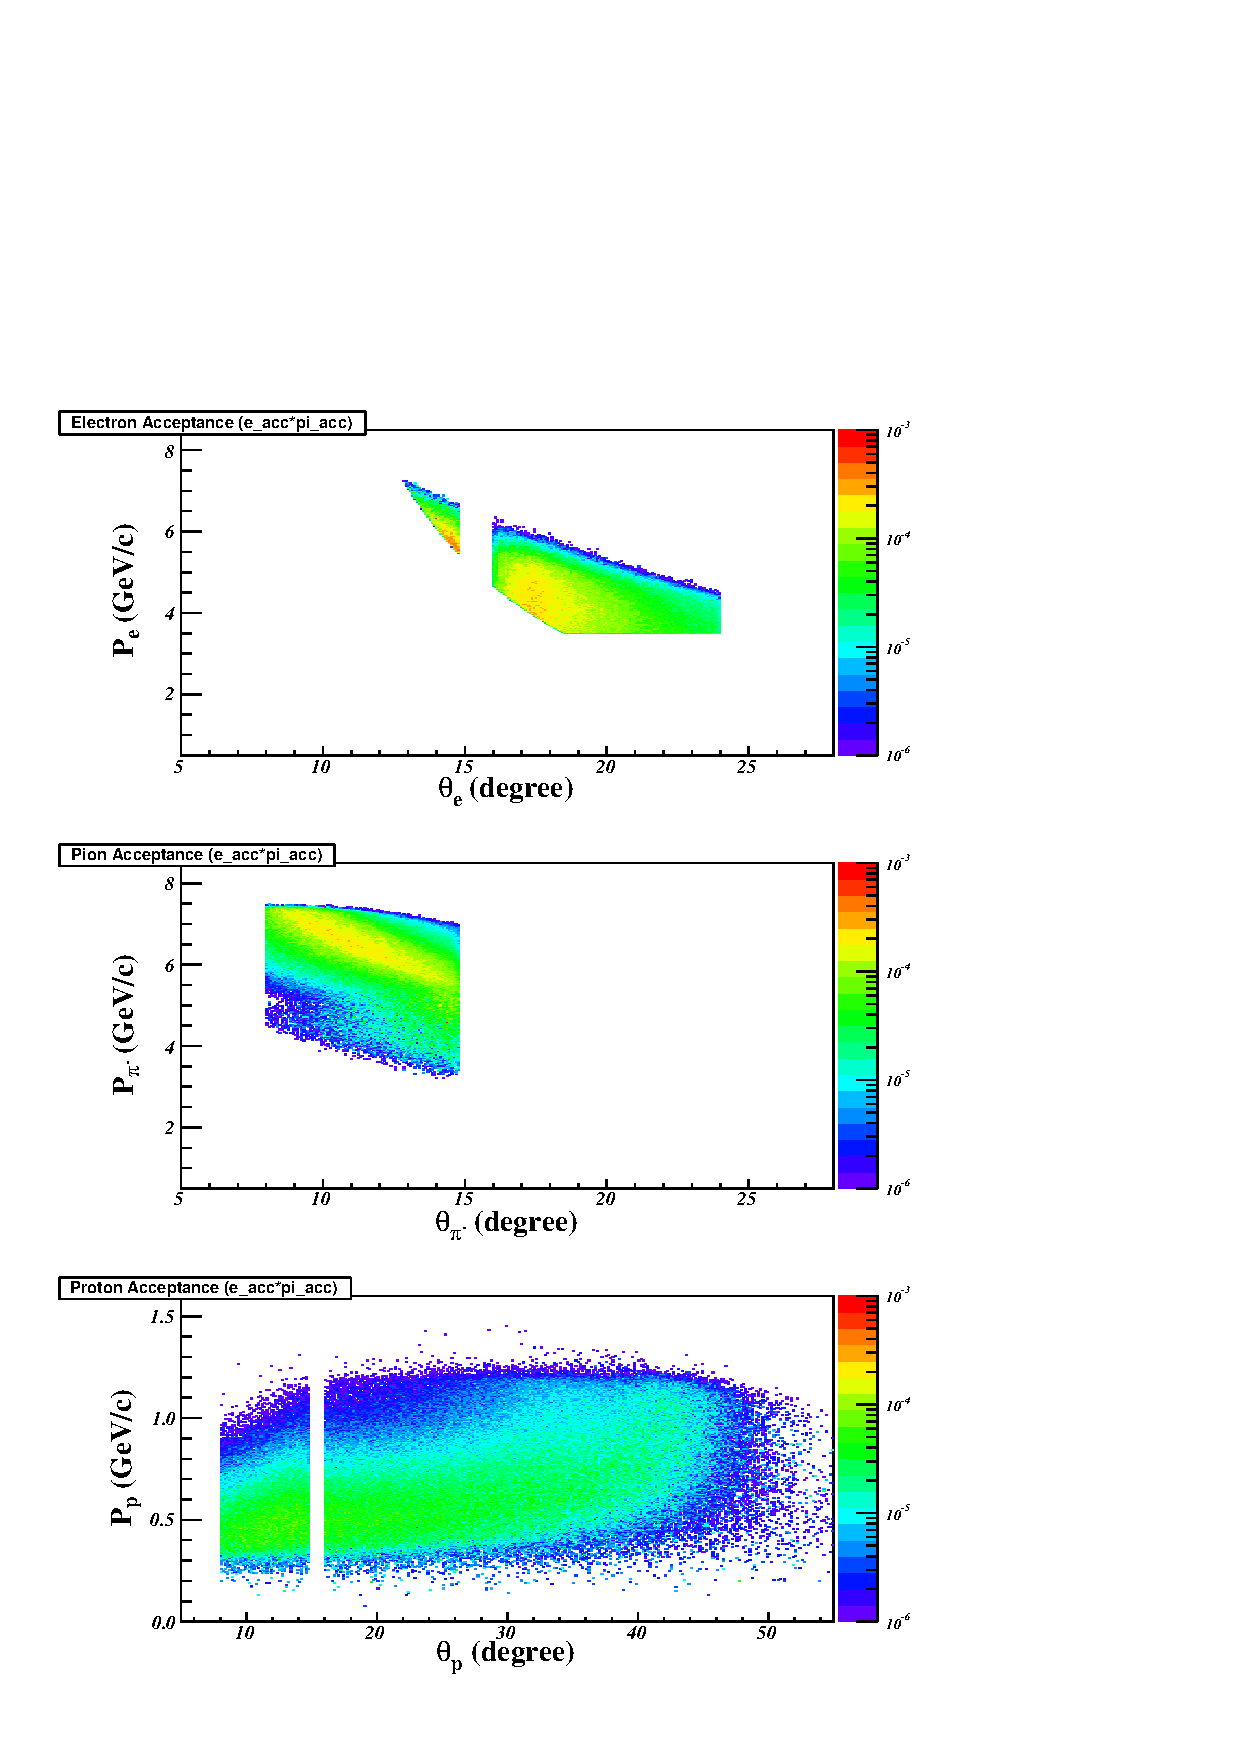
\includegraphics[type=pdf,
        ext=.pdf,read=.pdf,width=0.35\textwidth]{./figures/E11_acc_epi_Q2gt4}
    }
     \subfloat[w/o PRD]{
      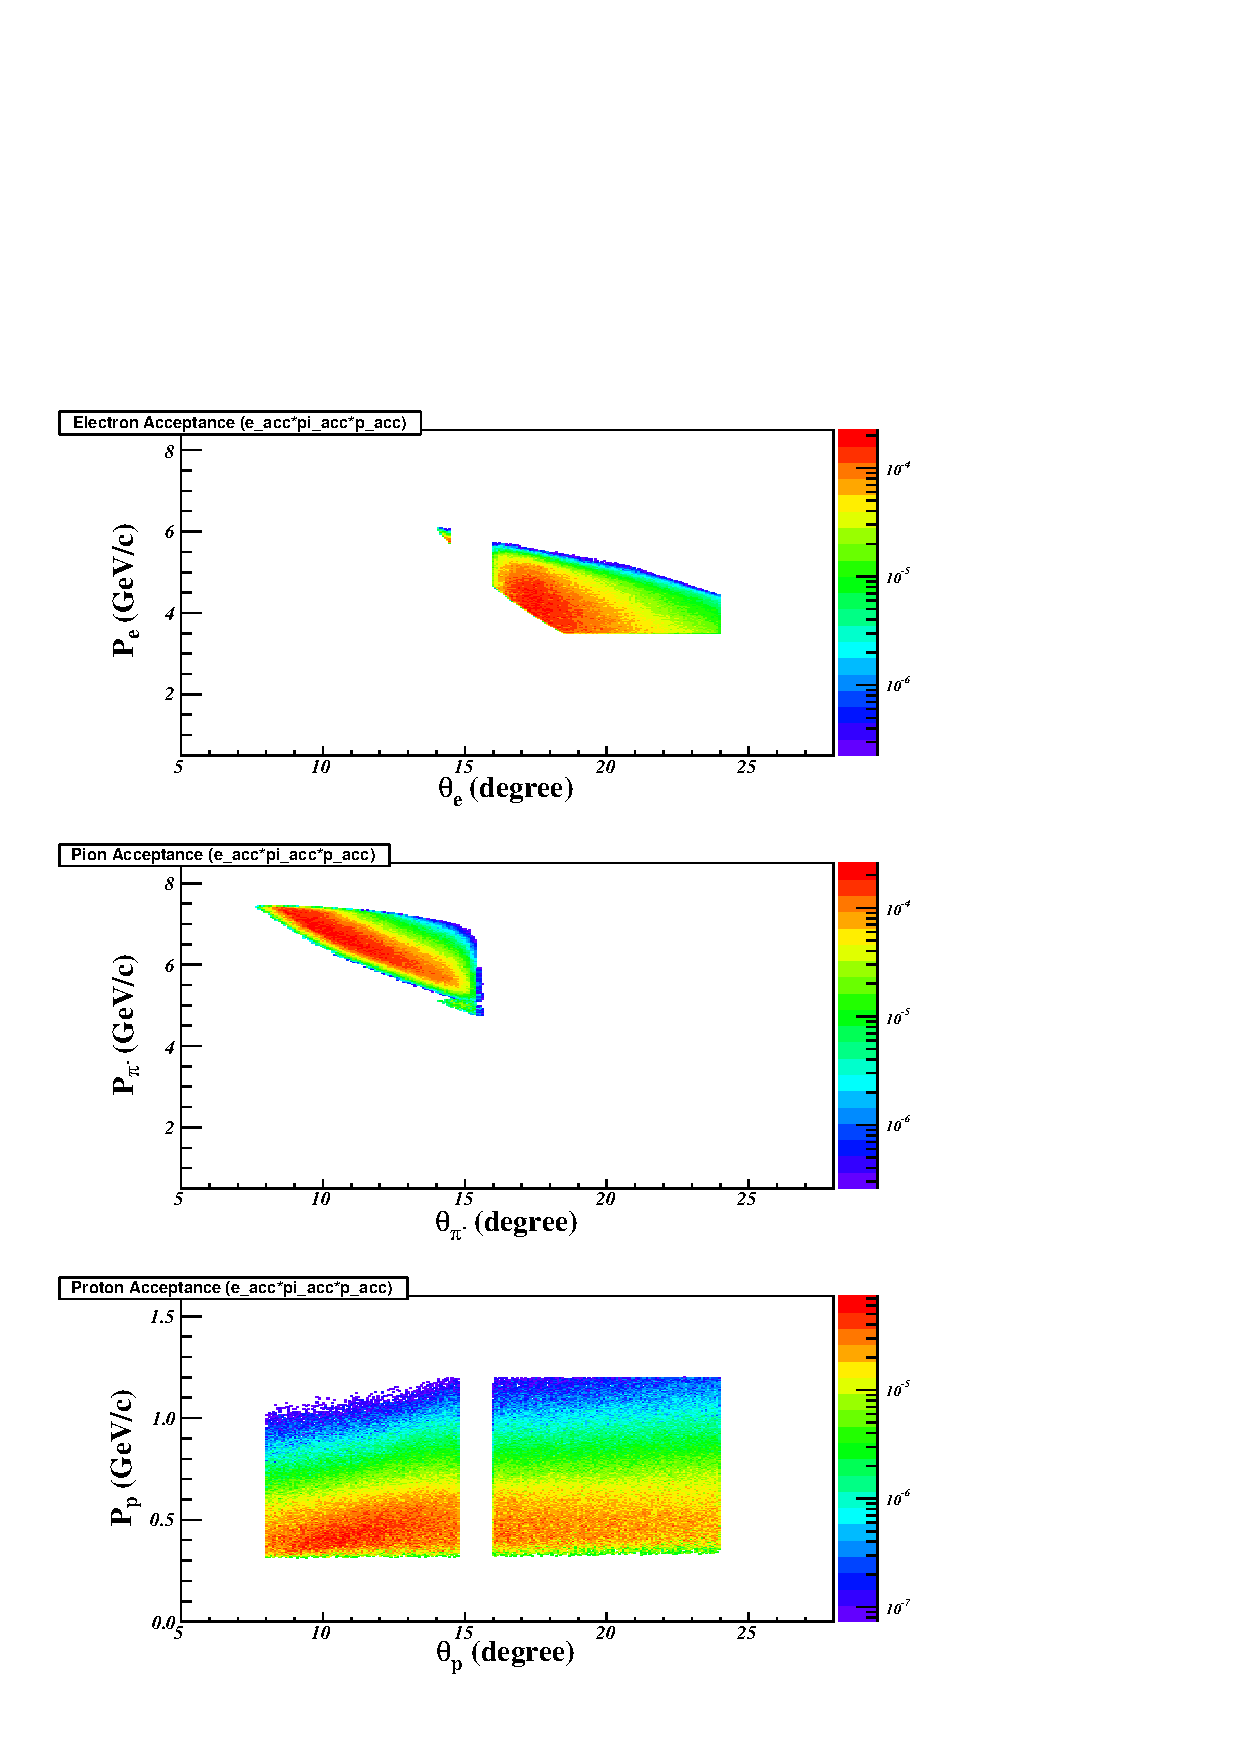
\includegraphics[type=pdf,
        ext=.pdf,read=.pdf,width=0.35\textwidth]{./figures/E11_acc_epip_Q2gt4}
    }
   \caption[The acceptance of the momenta and scattering angles for electrons,
     $\pi^{-}$ and protons]{\footnotesize{The acceptance of the momenta and
       polar angles w/ or w/o the PRD. In each panel, the top, middle and
       bottom plots are for electrons, $\pi^{-}$ and protons, respectively. A
       cut of $\mathrm{Q^{2}>4~GeV^{2}}$ is applied. Colors correspond to rates
       (Hz) in log scale.}}
  \label{p_theta}
  \end{center}
\end{figure}
The kinematic coverage in $Q^{2} vs. x_{B}$ is shown in Fig.~\ref{kin_cor}
where two proton detection cases were given: (a) by using existing SoLID
detectors to detect protons at small angles ($8^{\circ}\sim24^{\circ}$) and
adding a new proton recoil detector to detect rest of recoil protons at large
angle ($24^{\circ}\sim65^{\circ}$), or (b) by only using the existing SoLID
detectors. These distributions were weighted by the DEMP cross sections and the
spectrometer acceptance obtained from the GEANT4 simulation with the SIDIS
configuration. As shown in these plots, the range of $Q^{2}$ is from
1.0~GeV$^{2}$ to 8.0~GeV$^{2}$, $x_{B}$ goes from 0.1 up to 0.75.

Fig.~\ref{p_theta} shows the momentum and angular acceptance of electrons,
$\pi^{-}$ and protons which form the DEMP events and can be detected with the
SoLID detectors and (or) with the new PRD.  A cut of $\mathrm{Q^{2}>4~GeV^{2}}$
is applied since most of valid DEMP events are at high $Q^{2}$. The recoil
protons shown in Fig.~\ref{p_theta} have low momenta ranged from 0.3~GeV/c up
to 1.2~GeV/c and their rates distribute near uniformly along the scattering
angle.

\subsection{Estimated Rates}

\begin{table}[!ht]
\centering
\begin{tabular}{|c|c|c|}
 \hline
  $\mathrm{1<Q^{2}<4~GeV^{2}}$ & $\mathrm{Q^{2}>4~GeV^{2}}$ & Total\\
 \hline
\multicolumn{3}{|c|}{DEMP: $\vec{n}(e,e'\pi^{-}p)$ Triple-Coincidence (Hz)}\\
 \hline
 17.79 (0.22)   &  0.53 (0.31) & 26.45 (7.66)   \\
 \hline
\multicolumn{3}{|c|}{SIDIS: $\vec{n}(e,e'\pi^{-})X$ Double-Coincidence (Hz)}                                     \\
 \hline
        1388.85 & 35.77        & 1424.62   \\
 \hline
\end{tabular}
\caption[Triple-Coincidence rates for
  neutron-DEMP]{\footnotesize{Triple-Coincidence rates for DEMP events compared
    with the SIDIS rates. Numbers in brackets are the DEMP rates with only
    detecting protons using existing SoLID detectors. The online production
    trigger will be the SIDIS double-coincidence trigger of which rates are
    also given.}}
\label{rate_table}
\end{table} 
Table~\ref{rate_table} lists the triple-coincidence rate of the DEMP
events. The rates were calculated with the simulated events weighted by the
target luminosity, the SoLID acceptances and cross sections. The rates are the
unpolarized event rates and are not corrected by the beam and target
polarization, target dilution and so on. The total integrated physics rate is
estimated to be around 26~Hz at 11~GeV, or 0.53 Hz at
$\mathrm{Q^{2}>4~GeV^{2}}$. If only using the existing SoLID detectors to
detect protons, the rate drops to 0.31 Hz at $\mathrm{Q^{2}>4~GeV^{2}}$.  For
comparing, the table also gives the SIDIS rate which will be the online
production trigger rates and is the main background of the DEMP events.

\subsection{Asymmetry Projections}

\begin{figure}[!ht]
 \begin{center}
     \subfloat[w/ PRD]{
      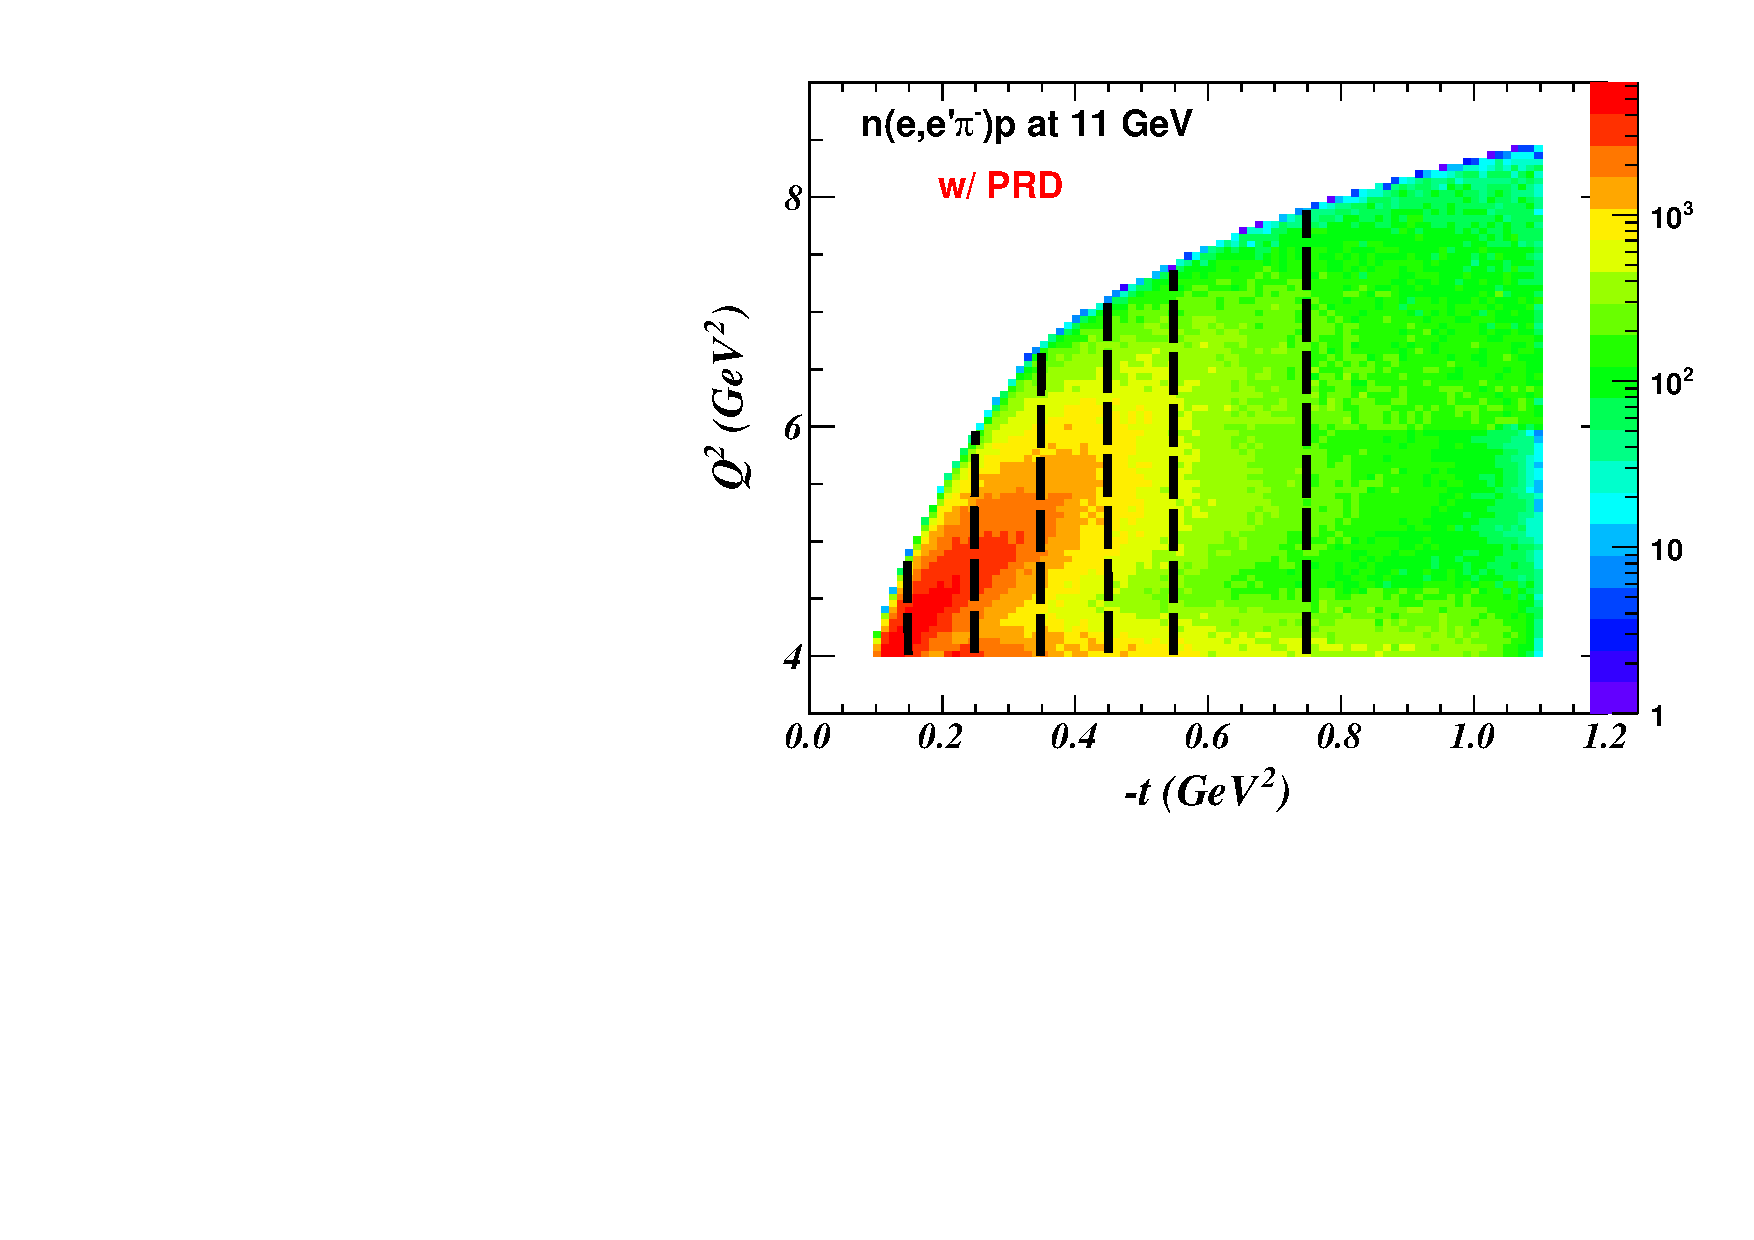
\includegraphics[type=pdf,
        ext=.pdf,read=.pdf,width=0.5\textwidth]{./figures/E11_Q2_t_bin_prd} }
    \subfloat[w/o PRD]{
      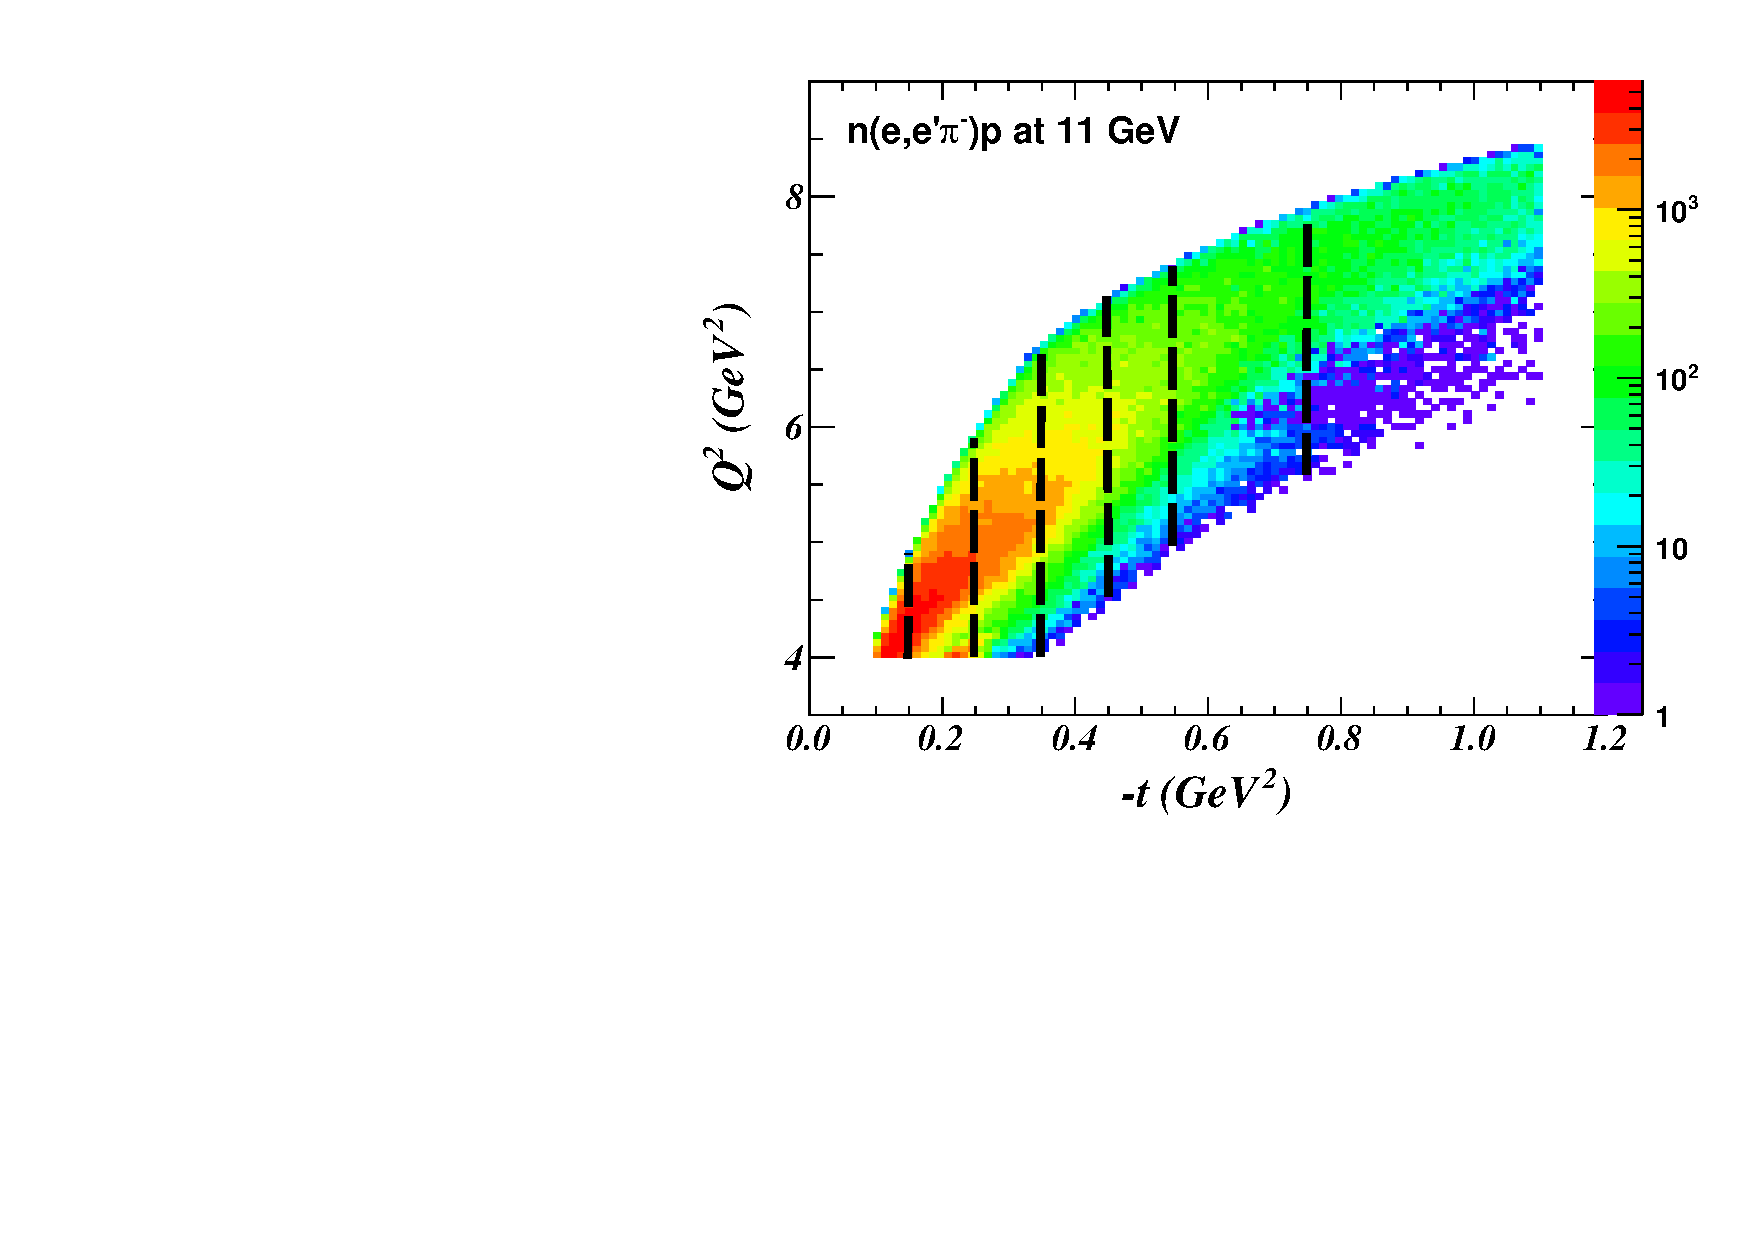
\includegraphics[type=pdf,
        ext=.pdf,read=.pdf,width=0.5\textwidth]{./figures/E11_Q2_t_bin} }
   \caption[$Q^{2}$ vs. $-t$]{\footnotesize{$Q^{2}$ vs. $-t$ where the black
       dash lines specify the boundaries of 7 $-t$ bins. The color panel
       indicates the raw counts with 48 days of beam time at 11!GeV and
       assuming protons to be detected only by existing SoLID detectors.}}
  \label{Q2_t_bin}
  \end{center}
\end{figure}

The proposed new experiment will run in parallel with E12-10-006 of which total
beam time of 48 days at $E_{0}$=11~GeV has been approved.  As shown in
Fig.~\ref{Q2_t_bin}, We defined 7 $-t$ bins of which the the boundaries are
defined by the array:
 \begin{equation}
     -t[8] = [0.0, 0.15, 0.25, 0.35, 0.45, 0.55, 0.75, 1.10]~~~~(in~GeV^{2})
 \end{equation}
The number of events ($N_{i}$) in the $i$th bin is calculated with the total
simulated events after applying cuts on important kinematic variables,
e.g. $Q^{2}>$4~GeV$^{2}, W>2~GeV, 0.55<\epsilon<0.75$ and $t_{min}<t<t_{max}$. As
shown in Eq.~\ref{ncount}, each event survived the cuts then is weighted by the
unpolarized cross section, the acceptance of the electron, pion and
photon. $N_{i}$ is further corrected by the phase-space ($PSF$) defined in the
event generator to randomly generate a total number of events ($N_{gen}$),
beam-time ($T$), the target luminosity ($L=10^{36} cm^{-2}s^{-1}$), and the
overall detector efficiency ( $\epsilon_{eff}$):
 \begin{equation}
     N_{i} = (\sum_{j\in i-bin} \sigma^{avg}_{j}\cdot A^{e}_{j} \cdot
     A^{\pi^{-}}_{j} \cdot A^{p}_{j}) \cdot (PSF/N_{gen}) \cdot T \cdot L \cdot
     \epsilon_{eff},
     \label{ncount}
 \end{equation}
where $j$ is the $j$th event in the $i$th bin, $\sigma^{avg}_{j}$ is the cross
section of the event. $A^{e(\pi^{-},p)}_{j}$ is the acceptance weight of the
electron (pion, proton) in this event. The detector efficiency,
$\epsilon_{eff}$, is fixed at 85\%. $N_{i}$ corresponds to the raw
experimental count of electrons scattering on neutrons in $\mathrm{^{3}He}$
before taking into account the target polarization ($P\sim60\%$), the
effective polarization of neutrons ($\eta_{n}\sim86.5\%$) and the dilution
effect from other reaction channels when electrons scattering on
$\mathrm{^{3}He}$ ($f \sim 90\%$). The statistical error of the target single
spin asymmetry ($A_{UT}$) in each bin can be given as:
  \begin{equation}
    \delta A_{UT} = \frac{1}{P\cdot\eta_{n}\cdot f} \sqrt{\frac{1-(P\cdot
        <A_{UT}>)^{2}}{N^{+}_{i}+N^{-}_{i}}},
    \label{stat_err}
 \end{equation}
where $N^{+(-)}_{i}$ is the number of counts in each bin when the target
polarization is up (down), and we easily have $N_{i}=N^{+}_{i}+N^{-}_{i}$;
$<A_{UT}>$ is the average asymmetry in the bin. As shown in Appendix.~A,
$A_{UT}$ is predicted with a phenomenological model, but because of not
performing a L/T separation in this experiment, the asymmetry should be
corrected by another dilution factor which is defined as:
\begin{equation}
  f_{L/T} =\frac{\epsilon\cdot\sigma_{L} }{\sigma_{T}+\epsilon\cdot\sigma_{L} },
\end{equation} 
where $\epsilon=1/(1+\frac{2\nu}{Q^{2}}tan^{2}(\theta))$
and additional dilution due to $\sigma_{TT}$ is assumed to be small. 
Hence, $A_{UT} = f_{L/T}\cdot A_{UT}^{model}$.

\begin{figure}[!ht]
 \begin{center}
      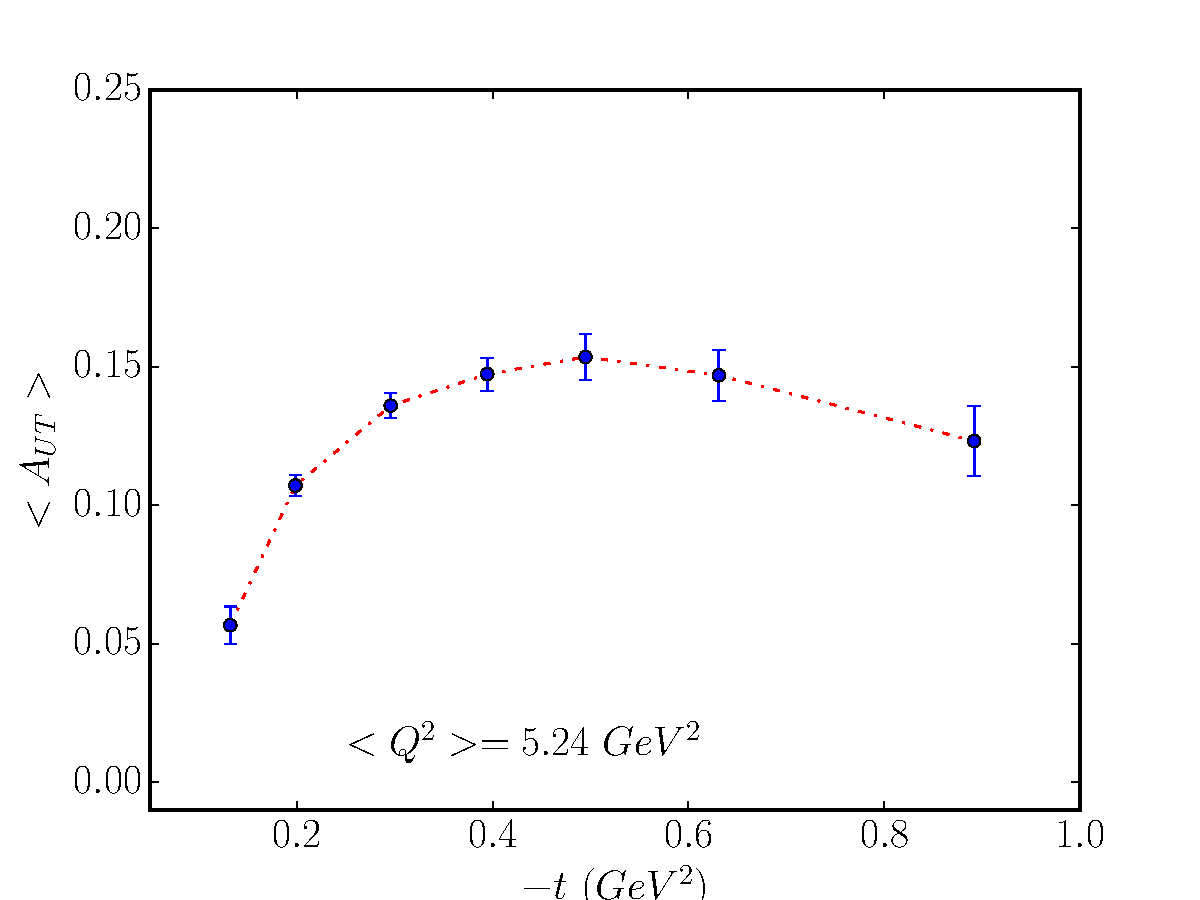
\includegraphics[type=pdf,
        ext=.pdf,read=.pdf,width=0.7\textwidth]{./figures/bin_asym_t}
      \caption{\footnotesize{Projection of target sing spin asymmetry
          ($A_{UT}$) in $-t$ binning for DEMP with transversely polarized
          $\mathrm{^{3}He}$ at $E_{0}$=11~GeV. The error bars are the projected
          statistical uncertainties defined in Eq.~\ref{stat_err}. The
          asymmetry value in each bin is predicted with the model given in Appendix. A and is diluted due to not separating the L/T
          contributions. The left plot shows the projection w/o a new proton
          recoil detector while the right plot shows a better ojected result
          with the new detector. One can see the average asymmetries are also
          changed between two configurations and it is because the asymmetry
          strongly depends on $Q^{2}$ which changes w/ or w/o the PRD.}}
  \label{asym_t}
  \end{center}
\end{figure}
Fig.~\ref{asym_t} shows the distribution of $A_{UT}$ vs. $-t$ with projected
statistical errors discussed above. Compared with the existing HERMES results
(Fig.~\ref{fig:hermes_aut}), the new measurement could provide more precious
data to be directly compared with theoretical predictions. The detailed information of each bin has been listed in Table~\ref{asym_bin_table}
	\begin{table}[!ht]
	\centering
	\begin{tabular}{|c|c|c|c|c|c|c|c|}
	   	\hline 
	w/ PRD   &  Bin\#1 & Bin\#2 & Bin\#3 & Bin\#4 & Bin\#5 & Bin\#6 & Bin\#7 \\
	 \hline
	  $<-t>$                &  0.13 & 0.20   & 0.30   & 0.40   & 0.50   & 0.64   & 0.90  \\
	   $<Q^{2}>$          & 4.22  & 4.59   & 5.02   & 5.38   & 5.64   & 5.90  & 6.27  \\
	   $<A_{UT}>$        &$6.53\times 10^{-2}$   & $1.51\times 10^{-1}$   & $2.06\times 10^{-1}$    & $2.30\times 10^{-1}$    & $2.38\times 10^{-1}$    & $2.20\times 10^{-1}$   & $1.47\times 10^{-1}$   \\
	   $\delta A_{UT}$  &  $6.50\times 10^{-3}$   & $3.15\times 10^{-3}$    &   $3.36\times 10^{-3}$  &  $4.05\times 10^{-3}$   &  $5.02\times 10^{-3}$   &   $4.64\times 10^{-3}$ &   $4.95\times 10^{-3}$ \\
	   $N$                     & $6.55\times 10^{4}$   &$2.78\times 10^{5}$   & $2.43\times 10^{5}$   &  $1.66\times 10^{5}$  & $1.08\times 10^{5}$  &  $1.27\times 10^{5}$ &$1.13\times 10^{5}$  \\
	 \hline
	 	\multicolumn{3}{c}{ } \\
	  \hline
	w/o PRD   &  Bin\#1 & Bin\#2 & Bin\#3 & Bin\#4 & Bin\#5 & Bin\#6 & Bin\#7 \\
	\hline 
	    $<-t>$                &  0.13 & 0.20   & 0.30   & 0.39   & 0.49   & 0.63   & 0.89  \\
	   $<Q^{2}>$          & 4.22  & 4.67   & 5.23   & 5.78   & 6.26   & 6.81  & 7.59  \\
	   $<A_{UT}>$        &$5.67\times 10^{-2}$   & $1.07\times 10^{-1}$   & $1.36\times 10^{-1}$    & $1.47\times 10^{-1}$    & $1.54\times 10^{-1}$    & $1.47\times 10^{-1}$   & $1.23\times 10^{-1}$   \\
	   $\delta A_{UT}$  &  $6.76\times 10^{-3}$   & $3.73\times 10^{-3}$    &   $4.42\times 10^{-3}$  &  $5.92\times 10^{-3}$   &  $8.30\times 10^{-3}$   &   $9.15\times 10^{-3}$ &   $1.26\times 10^{-2}$ \\
	   $N$                     & $6.07\times 10^{4}$   &$1.99\times 10^{5}$   & $1.41\times 10^{5}$   &  $7.87\times 10^{4}$  & $4.00\times 10^{4}$  &  $3.29\times 10^{4}$ &$1.75\times 10^{4}$  \\
	 \hline
	\end{tabular}
	\caption[Detailed information of projected bins]{\footnotesize{Detailed information of projected bins from the new DEMP measurements with SoLID, while $<Q^{2}>$ and $<-t>$ are in the unit of $GeV^{2}$. The top (bottom) table is with respect to the case of proton detection w/ (w/o) a new PRD.}}
	\label{asym_bin_table}
\end{table} 

\section{Missing Mass and Background}
The dominated background of the DEMP measurements comes from the SIDIS reactions of electrons scattering on the neutron and two protons in $\mathrm{^{3}He}$. In addition to detect the recoil proton, we also rely on reconstructing the neutron missing mass spectrum to ensure the exclusivity of the DEMP events. In SIDIS, however, the final states include the scattered electron, the hadrons ($\pi^{\pm}$, $K^{\pm}$ etc.), as well as the undetected target fragments which could contain protons. 

We studied the contamination of the SIDIS events in the DEMP missing mass spectrum. The SIDIS reactions, $p(e,e'\pi^{-})X$ and $n(e,e'\pi^{-})X$,  were simulated with the same generator used for the SoLID-SIDIS proposals, and their rates were calculated by matching the acceptance of scattered electrons and pions with the ones in DEMP. It is difficult to estimate how many percentage of the SIDIS target fragments contain protons, so we assumed the target fragments ("X") all contain one or more protons. This conservative assumption would cause the SIDIS rate being significantly overestimated. 

However, considering other proton channels (like proton-knock-out during QE) and accidental events, it may still be a good estimation, although I would expect the SIDIS peak would be much broader.

\begin{figure}[!ht]
 \begin{center}
     \subfloat[w/ PRD]{
      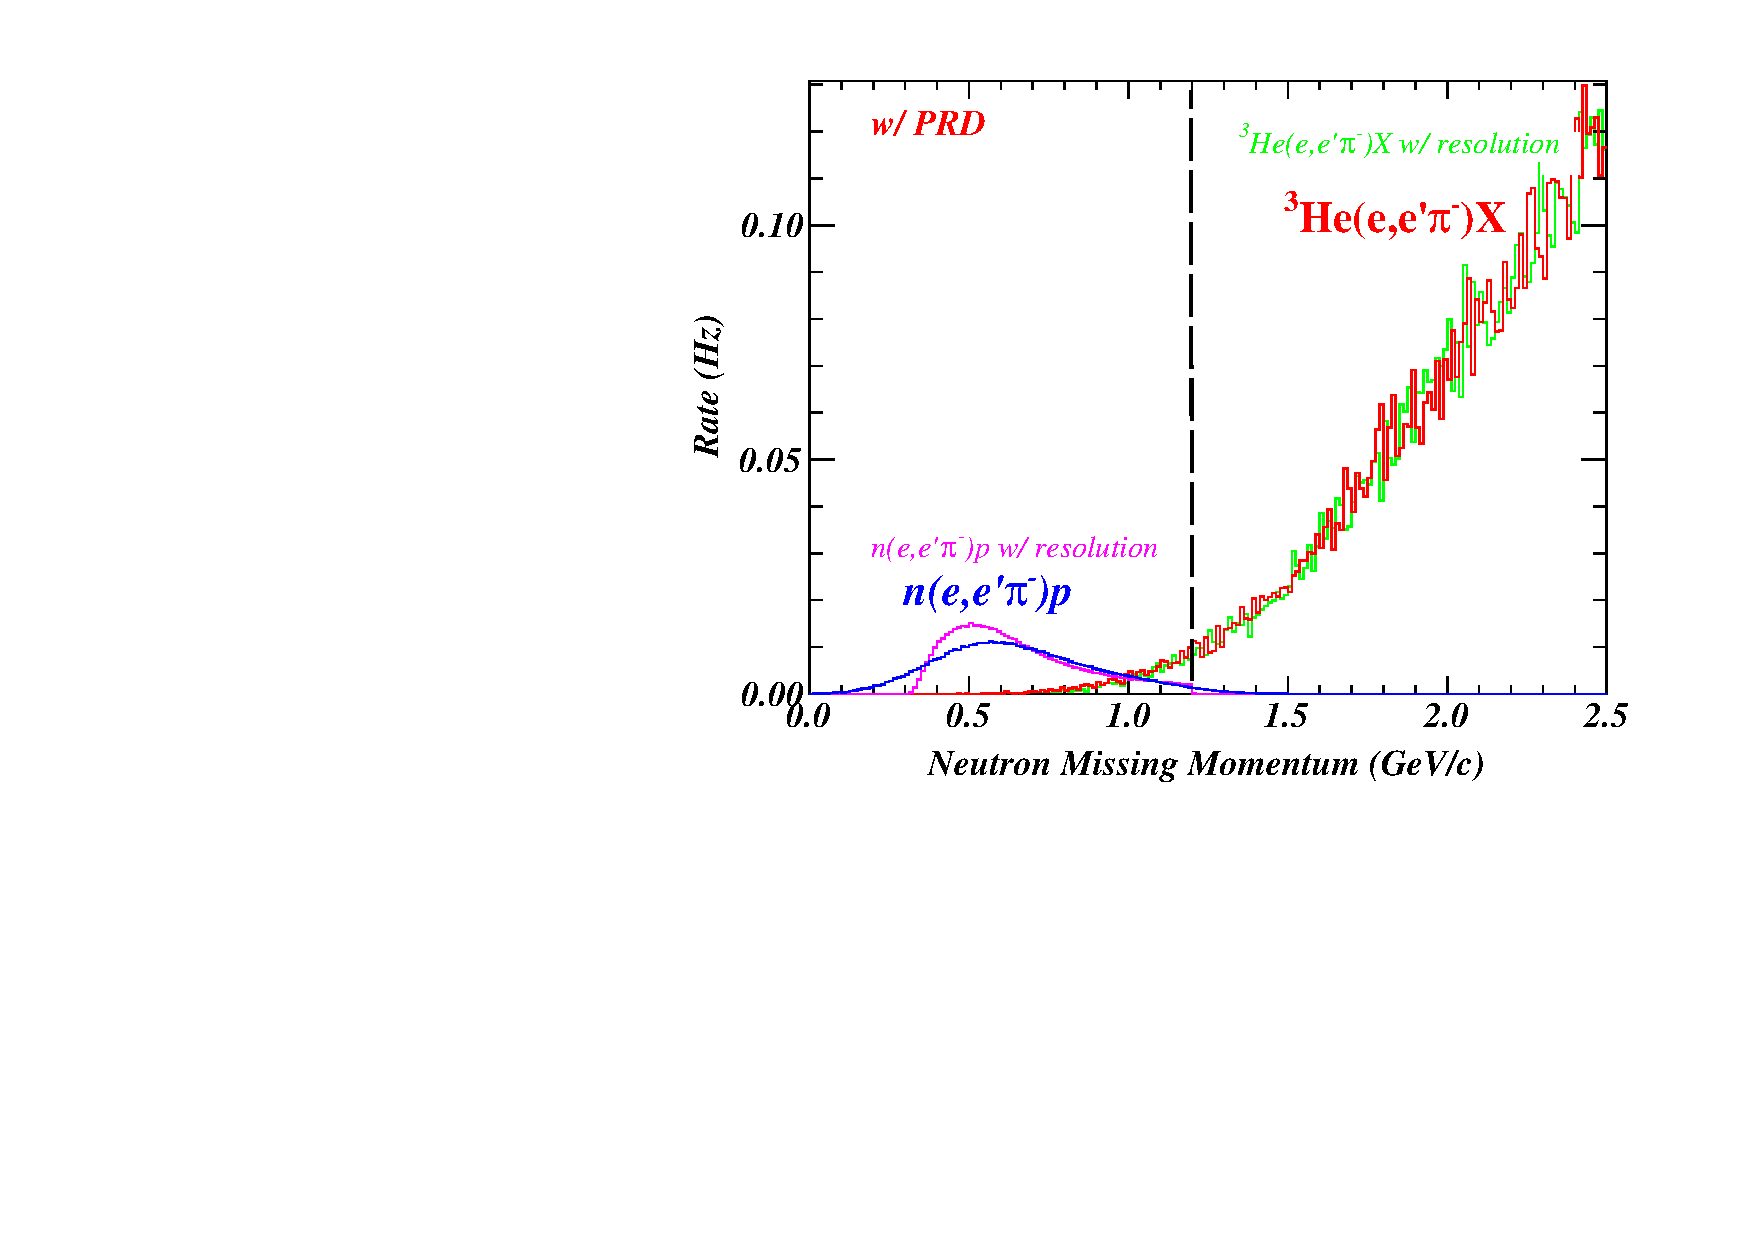
\includegraphics[type=pdf,ext=.pdf,read=.pdf,width=0.5\textwidth]{./figures/Missing_P_prd_nolog} }
    \subfloat[w/o PRD]{
      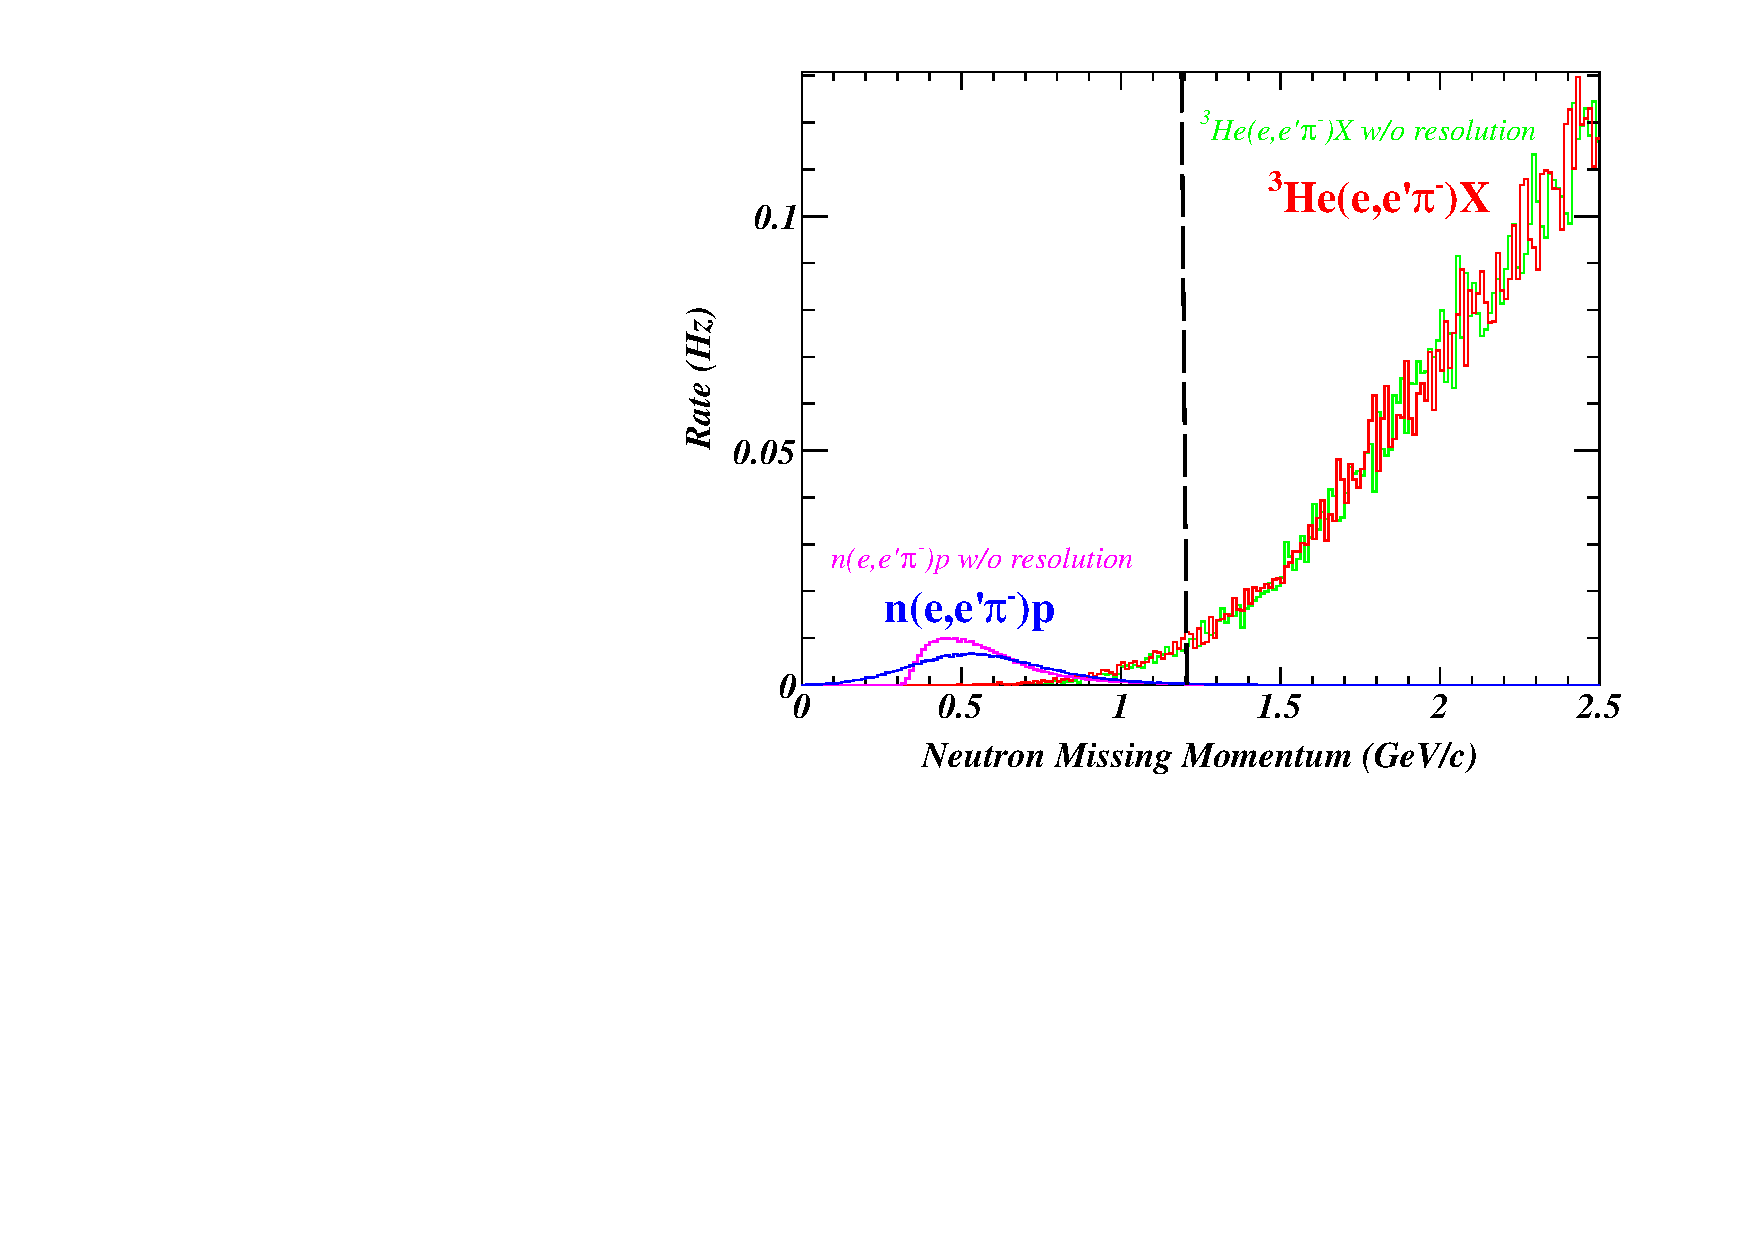
\includegraphics[type=pdf,ext=.pdf,read=.pdf,width=0.5\textwidth]{./figures/Missing_P_nolog} }
   \caption[Missing Momentum]{\footnotesize{Missing momentum spectra of DEMP and SIDIS events. The missing momentum distributes are well separated between two processes and one can apply a cut at $P_{miss}<1.2~GeV/c$ (indicated by the black dash line) to remove most of SIDIS events.}}
  \label{missing_mom}
  \end{center}
\end{figure}
Shown in Fig.~\ref{missing_mom}, we reconstruct the missing momenta of both the DVMP and SIDIS processes and immediately discovered that the missing momentum distributions of two processes are well separated. The SIDIS background will be largely rejected when we apply a cut, $P_{miss}<1.2~GeV/c$. 

\begin{figure}[!ht]
 \begin{center}
     \subfloat[w/ PRD]{
      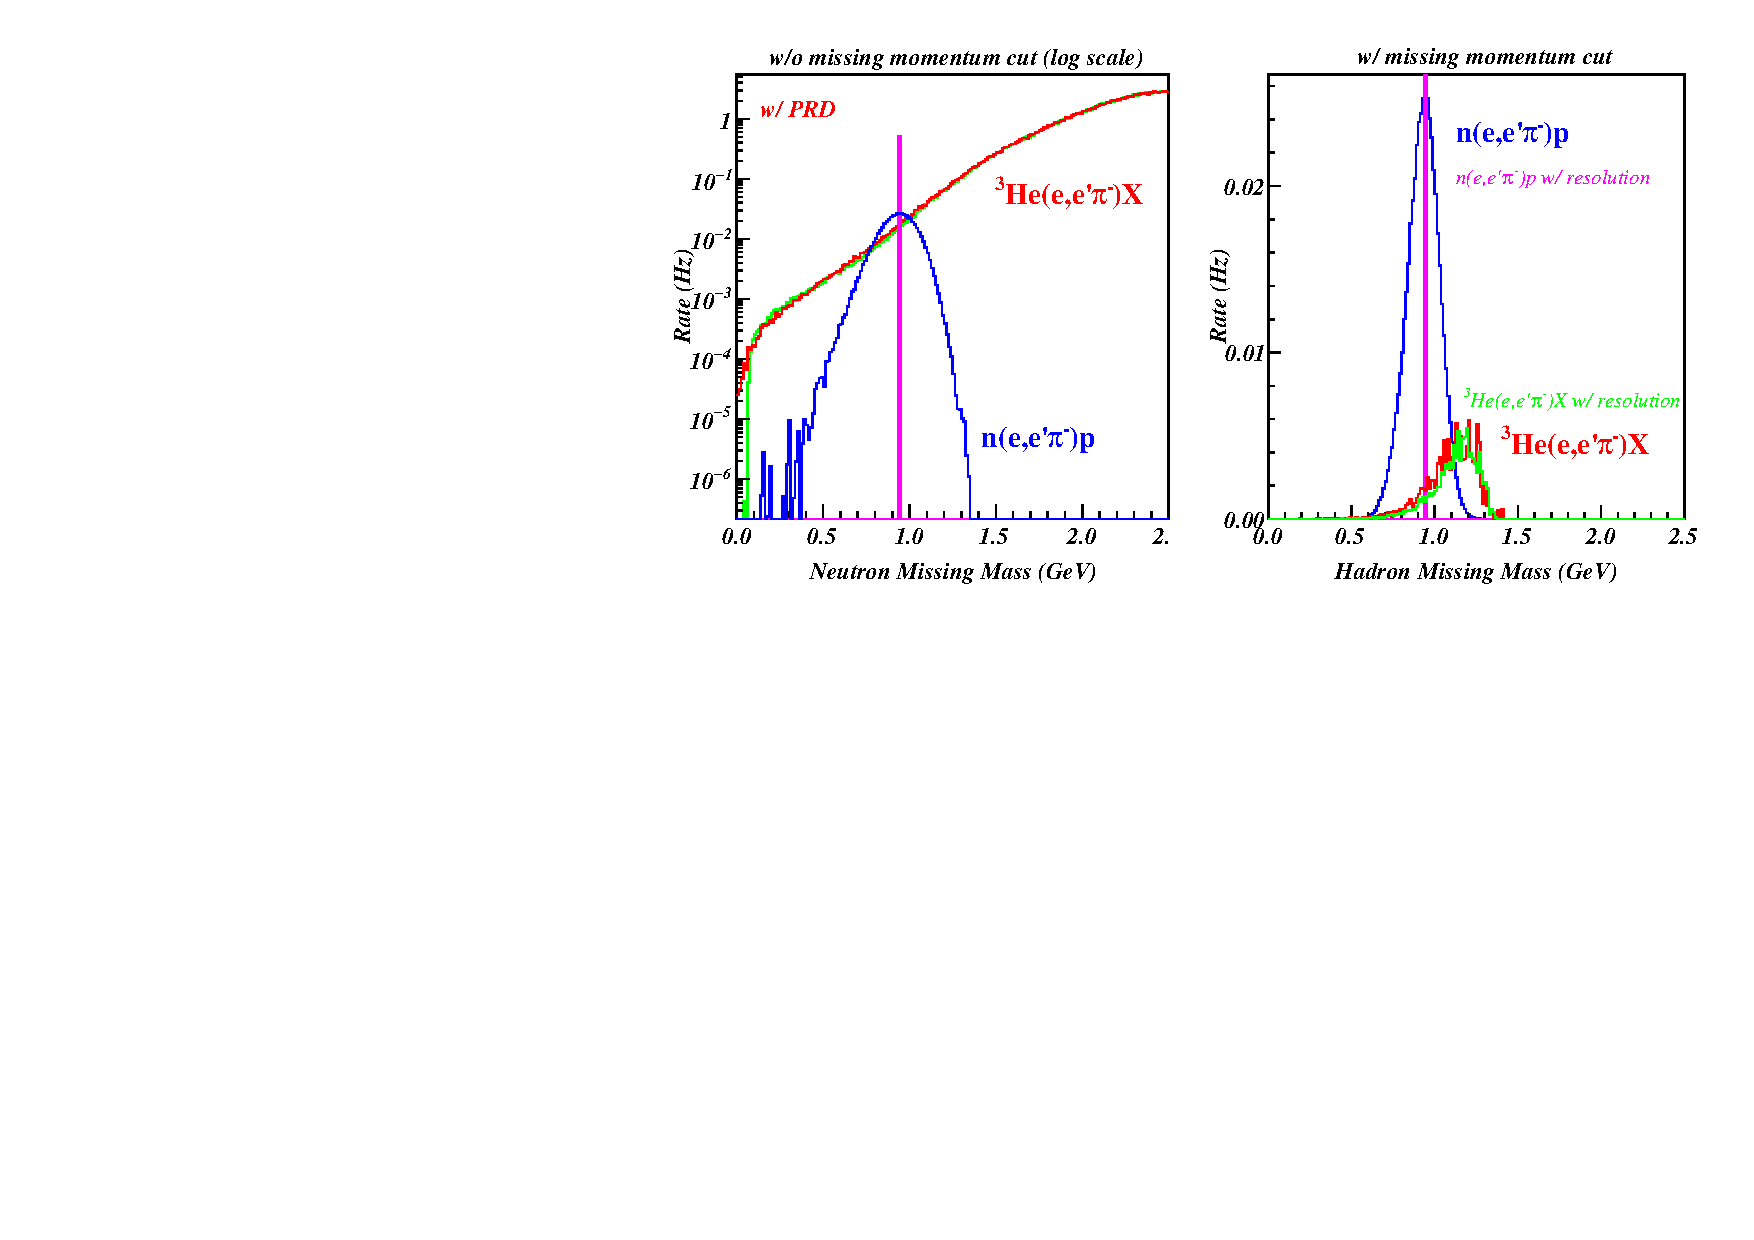
\includegraphics[type=pdf,
        ext=.pdf,read=.pdf,width=0.85\textwidth]{./figures/Missing_Mass_cut_prd} } \\
    \subfloat[w/o PRD]{
      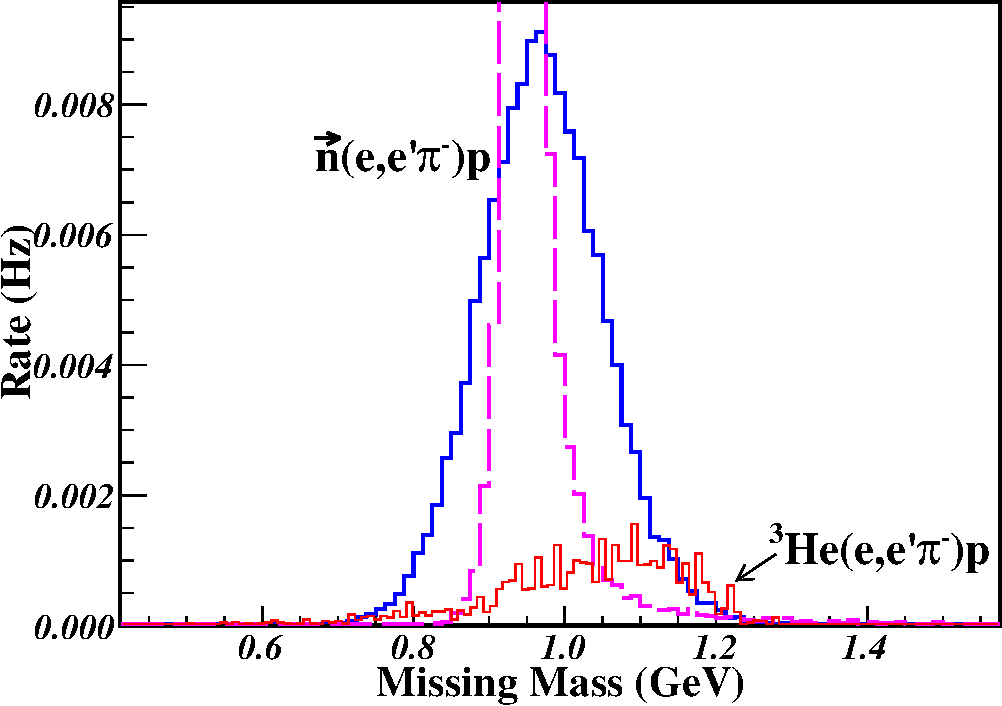
\includegraphics[type=pdf,
        ext=.pdf,read=.pdf,width=0.85\textwidth]{./figures/Missing_Mass_cut} }
   \caption[Missing Mass]{\footnotesize{Missing mass spectra of DEMP and SIDIS events. Top (bottom) panel shows the missing mass distribution of DEMP events w/ (w/o) proton detection by a new PRD. The left (right) plot of each panel shows the background contamination from SIDIS events before (after) the missing momentum cut shown in Fig.~\ref{missing_mom}. The SIDIS background is already small compared with DEMP events. The actual SIDIS background should be much smaller, since we overestimated the SIDIS rate by assuming all target fragments ("X") in the SIDIS process contain protons.}}
  \label{missing_mass}
  \end{center}
\end{figure}

We then reconstructed the missing mass spectra of the DEMP and SIDIS events w/ and w/o the missing momentum cuts, shown in Fig.~\ref{missing_mass}. Befor applying the missing momentum cut, the SIDIS background overwhelms the DVMP peak (but note that the SIDIS rate is overestimated). When applying the cut, the DVMP peak dominates and the SIDIS background is largely suppressed. If we consider the fact that not every "X" in SIDIS contains a proton, the background should be negligible. 

\section{Systematic Uncertainties}
\begin{table}[!htp]
\centering
\begin{tabular}{|c|c|}
\hline
{\bf Sources}                  & {\bf Relative Value} \\\hline
Beam Polarization         & $2\%$ \\\hline 
Target Polarization         & $3\%$ \\\hline 
Acceptance                    & $3\%$ \\\hline
Other Contamination      & $<5\%$ \\\hline
Radiation Correction      & $1\%$ \\\hline
\end{tabular}
\caption{\footnotesize{Expected systematic errors.}}\label{table:det_sys_err}
\end{table}
The detector related systematic errors are expected to be similar to the ones
given in the E12-10-006 proposal as well as in other SIDIS experiments with
SoLID, as shown in Table~\ref{table:det_sys_err}. 
